\begin{enumerate}
\item Obtain the Boolean Expression for the Logic circuit shown below
\label{prob:2013/c/6/b}
\hfill (CBSE 2013)
	\usetikzlibrary{circuits.logic.IEC,calc}

	   \begin{circuitikz} \draw
(0,2) node[or port]  (myor1) {}
(0,0) node[and port] (myand) {}
(2,1) node[or port] (myor2) {}
(myor1.out) -- (myor2.in 1)
(myand.out) -- (myor2.in 2);

\node[left] at (myor1.in 1) {\(X\)};
\node[left] at (myor1.in 2) {\(Y\)};
\node[left] at (myor1.in 1)[ocirc] {};
\node[left] at (myand.in 2) [ocirc] {};
\node[left] at (myand.in 1) {\(Y\)};
\node[left] at (myand.in 2) {\(Z\)};
\node[right] at (myor1.out) {};
\node[right] at (myand.out) {};

\node[right] at (myor2.out) {F};
\end{circuitikz}
\item Verify the Boolean Expression 
\label{prob:2013/c/6/a}
\hfill (CBSE 2013)
		\begin{align}
\label{eq:2013/c/6/a}
	               A+C=A+A'C+BC
		\end{align}
\item Draw the Logic Circuit for the following Boolean Expression 
\label{prob:2015-1/c/6/b}
\hfill (CBSE 2015)
		\begin{align}
\label{eq:2015-1/c/6/b}
f(x,y,z,w) = (x'+y)z + w'
		\end{align}
\item Verify the following
\label{prob:2015-1/c/6/a}
\hfill (CBSE 2015)
		\begin{align}
\label{eq:2015-1/c/6/a}
U' + V = U'V' + U'V+UV
		\end{align}
\item Draw the Logic Circuit for the given Boolean Expression
\label{prob:2015/c/6/b}
\hfill (CBSE 2015)
		\begin{align}
\label{eq:2015/c/6/b}
(U + V')W' + Z
		\end{align}
\item 
Verify the following using Boolean Laws
\label{prob:2015/c/6/a}
\hfill (CBSE 2015)
		\begin{align}
\label{eq:2015/c/6/a}
X+Y' = XY+XY'+X'Y'
		\end{align}
\item 
\label{prob:2016/c/6/b}
Write the Boolean Expression for the result of the Logic Circuit as shown in Fig.  
\ref{fig:2016/c/6/b}
\hfill (CBSE 2016)
\begin{figure}
\centering
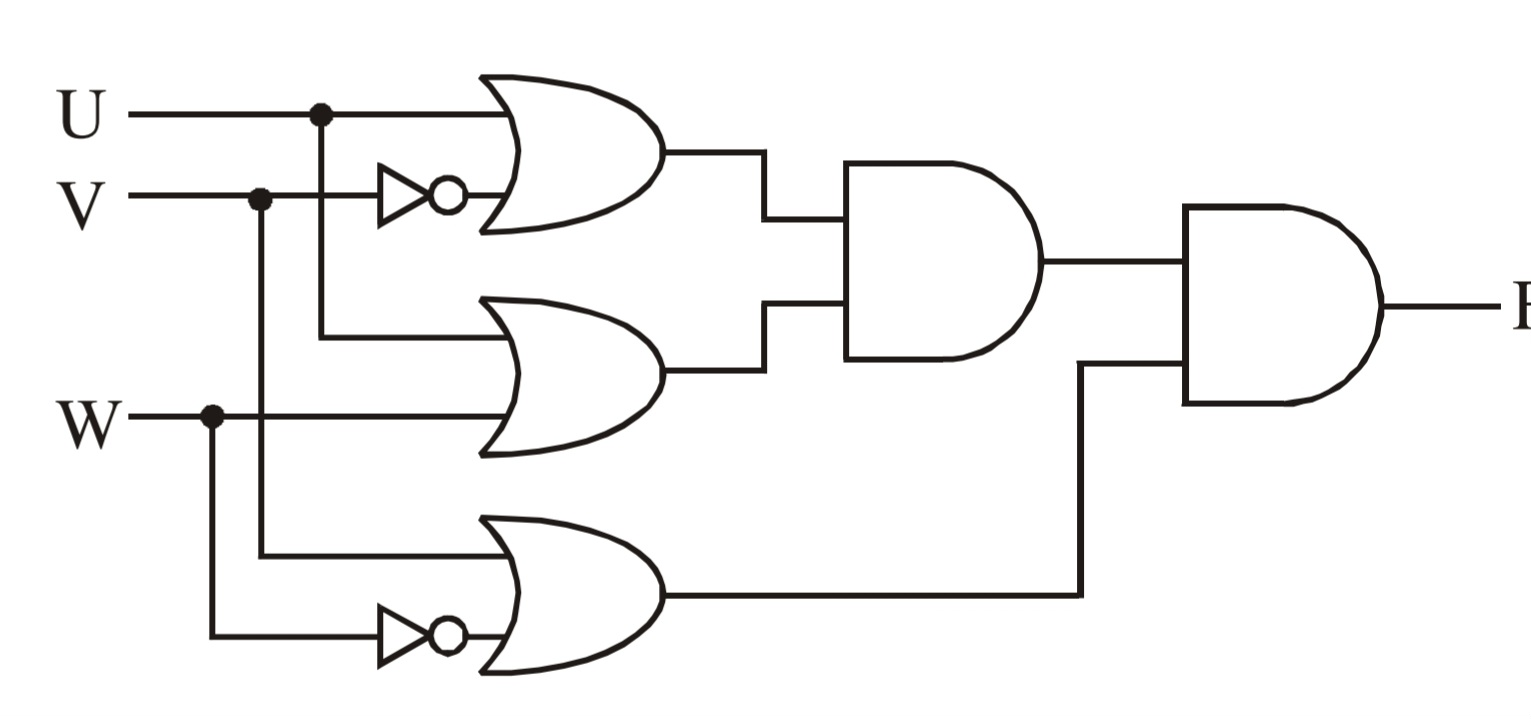
\includegraphics[width=\columnwidth]{figs/cbse-2016.jpg}
\caption{}
\label{fig:2016/c/6/b}
\end{figure}
\item Draw the logic circuit of the following Boolean Expression using only NAND Gates.
\hfill (CBSE 2017)
\label{prob:2017-1/c/6/b}
		\begin{align}
\label{eq:2017-1/c/6/b}
 XY + YZ
		\end{align}
\item Draw the Logic Circuit of the following Boolean Expression using only NOR Gates  
\hfill (CBSE 2017)
\label{prob:2017/c/6/b}
      \begin{align}
      (A+B)(C+D)
      \end{align}
\item Draw the Logic Circuit of the following Boolean Expression\hfill (CBSE 2018)
\begin{equation} 
(U'+V)(V'+W')
\end{equation}
\label{prob:2018/c/6/b}
\item Derive a Canonical POS expression for a Boolean function F, represented by 
Table \ref{tab:2019/c/6/c}\hfill (CBSE 2019)
\label{prob:2019/c/6/c}
\begin{table}[H]
\centering
\begin{tabular}{|l|l|l|c|}
	\hline
	X&Y&Z&F(X,Y,Z)\\
	\hline
	0&0&0&1\\
	0&0&1&0\\
	0&1&0&1\\
	0&1&1&0\\
	1&0&0&1\\
	1&0&1&1\\
	1&1&0&0\\
	1&1&1&0\\
	\hline
\end{tabular}
\caption{}
\label{tab:2019/c/6/c}
\end{table}
\item For the logic circuit shown in Fig.\ref{fig:2000/gate/ec/2/7}, find the simplified Boolean expression for the output. 
\label{prob:2000/gate/ec/2/7}
\hfill (GATE EC 2000)
\begin{figure}[H]
    \centering
    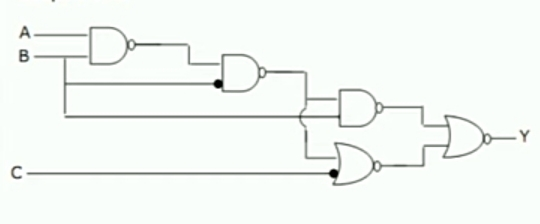
\includegraphics[width=\columnwidth]{figs/2000-gate-ec-2-7.jpg}
    \caption{}
\label{fig:2000/gate/ec/2/7}
\end{figure}
\item 
Obtain the Boolean Expression for the Logic circuit shown below
\label{prob:1993/gate/ec/4/8}
\hfill (GATE EC 1993)
	  	
	   \begin{circuitikz} \draw
(0,2) node[nand port] (mynand1) {}
(2,3) node[nand port] (mynand2) {}
(0,0) node[nand port] (mynand) {}
(2,-1) node[nand port] (mynand3) {}
(2,1) node[or port] (myor1) {}
(4,1) node[or port,number inputs =3] (myor2) {}
(mynand1.out) -- (myor1.in 1)
(mynand.out) -- (myor1.in 2)
(mynand2.out) -- (myor2.in 1)
(mynand3.out) -- (myor2.in 3)
(myor1.out) -- (myor2.in 2);
\node[left] at (mynand1.in 1) {\(A\)};
\node[left] at (mynand1.in 2) {\(B\)};
\node[left] at (mynand2.in 1) {\(A\)};
\node[left] at (mynand2.in 2) {\(A\)};
\node[left] at (mynand3.in 1) {\(C\)};
\node[left] at (mynand3.in 2) {\(C\)};
\node[left] at (mynand1.in 1)[ocirc] {};
\node[left] at (mynand.in 2) [ocirc] {};
\node[left] at (mynand.in 1) {\(B\)};
\node[left] at (mynand.in 2) {\(C\)};
\node[right] at (mynand1.out) {};
\node[right] at (mynand.out) {};
\node[right] at (mynand2.out) {};
\node[right] at (mynand3.out) {};
\node[right] at (myor2.out) {\(Y\)};
\end{circuitikz}
%
\item Implement Table
\ref{tab:1993/gate/ec/6/13}
using XNOR logic.
\label{prob:1993/gate/ec/6/13}
\hfill (GATE EC 1993)
\begin{table}[H]
	\centering
	\begin{tabular}{|c|c|c|}
		\hline
		\textbf{A}&\textbf{B}&\textbf{Y}\\
		\hline
		0&0&1\\
		\hline
		0&1&0\\
		\hline
		1&0&0\\
		\hline
		1&1&1\\   
		\hline 
	\end{tabular}
	\caption{}
\label{tab:1993/gate/ec/6/13}
\end{table}
\item 
\label{prob:1999-gate-ec-2-11}
For a binary half-sub-tractor having two inputs A and B, find the correct set of logical expressions for the outputs D (=A minus B) and X (=borrow).
\hfill (GATE EC 1999)
%
\item 
\label{prob:2007-gate-ec-43}
Find $X$ in the following circuit in Fig.
\ref{fig:2007-gate-ec-43}
\hfill (GATE EC 2007)
\begin{figure}[H]
\centering
	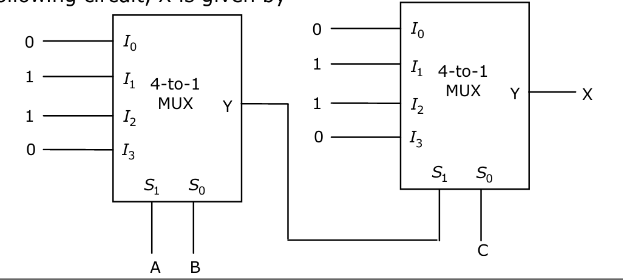
\includegraphics[width=1\columnwidth]{figs/2007-gate-ec-43.png}
\caption{}
\label{fig:2007-gate-ec-43}
\end{figure}
\item 
\label{prob:2007-gate-in-10}
      A logic circuit implements the boolean function F=X'.Y+X.Y'.Z'. It is found that the input combination X=Y=1 can never occur. Taking this into account, find a simplified expression for F. 
\hfill (GATE IN 2007)
\item 
\label{prob:2010-gate-ec-39}
Find the Boolean logic realised by the following circuit in Fig.
\ref{fig:2010-gate-ec-39}
\hfill (GATE EC 2010)
\begin{figure}[H]
\centering
	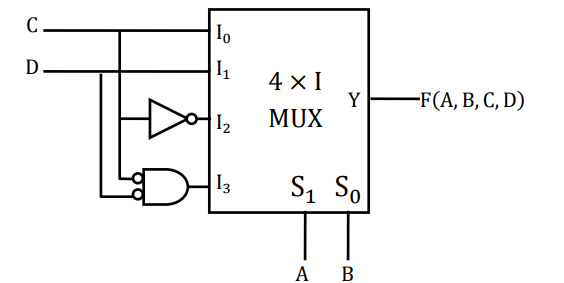
\includegraphics[width=1\columnwidth]{figs/2010-gate-ec-39.png}
\caption{}
\label{fig:2010-gate-ec-39}
\end{figure}
\item 
\label{prob:2011-gate-ec-20}
Find the logic function implemented by the circuit given below 
in Fig.
\ref{fig:2011-gate-ec-20}
\hfill (GATE EC 2011)
\begin{figure}[H]
\centering
	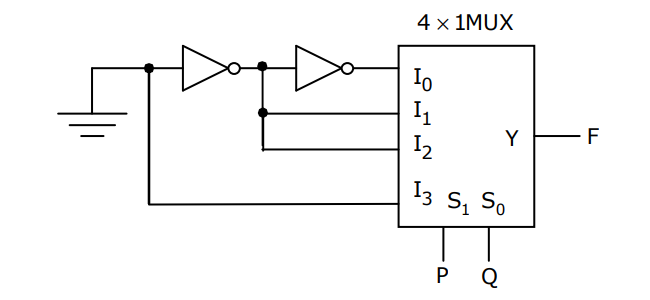
\includegraphics[width=\columnwidth]{figs/2011-gate-ec-20.png}
\caption{}
\label{fig:2011-gate-ec-20}
\end{figure}
\item
\label{prob:2016/gate/in/19}
Find F in the Digital Circuit given in the figure below
in Fig. \ref{fig:2016/gate/in/19}.
\hfill (GATE IN 2016)
\begin{figure}[H]
	\centering
\begin{tikzpicture}
 

 
% Logic ports
\node[nand port] (a) at (2,1){};
\node[nand port] (b) at (2,4){};
\node[nand port] (c) at (4,0){};
\node[nand port] (d) at (6,3){};

 
% Connection

 
\draw (a.in 2) -| (b.in 2);
\draw (b.out) -| (d.in 1);
 
\draw (a.out) -|  (c.in 1);
\draw (c.out) -| (d.in 2);
\draw (d.out) -- ++(1,0) node[near end,above]{F};
 
\draw (b.in 1) -- ++(-1.5,0)node[left](In1){X};
\draw (b.in 2) -- ++(-1.5,0)node[left](In3){Y};
\draw (c.in 2) -- ++(-1.5,0)node[left](In3){Z};
% Jump crossing element
1
\end{tikzpicture}
	\caption{}
\label{fig:2016/gate/in/19}
\end{figure}


\item 
\label{prob:2017-gate-ec-16}
Find the logic function implemented by the circuit given below 
in Fig.
\ref{fig:2017-gate-ec-16}
\hfill (GATE EC 2017)
\begin{figure}[H]
\centering
	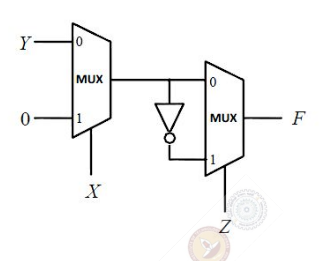
\includegraphics[width=\columnwidth]{figs/2017-gate-ec-16.png}
\caption{}
\label{fig:2017-gate-ec-16}
\end{figure}
\item 
\label{prob:2018-gate-ec-31}
Find the logic function implemented by the circuit given below 
in Fig.
\ref{fig:2018-gate-ec-31}
\hfill (GATE EC 2018)
\begin{figure}[H]
\centering
	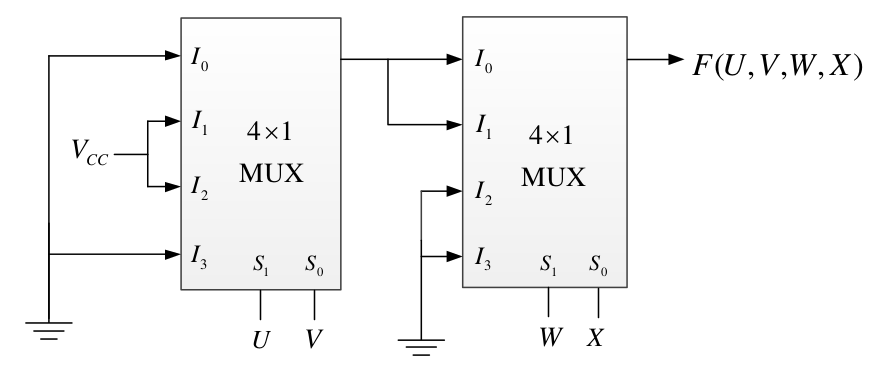
\includegraphics[width=\columnwidth]{figs/2018-gate-ec-31.png}
\caption{}
\label{fig:2018-gate-ec-31}
\end{figure}
\item 
\label{prob:2018-gate-ee-14}
Find the logic function implemented by the circuit given below 
in Fig.
\ref{fig:2018-gate-ee-14}
\hfill (GATE EE 2018)
\begin{figure}[H]
\centering
	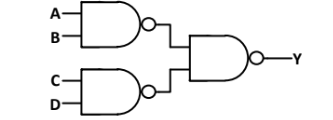
\includegraphics[width=\columnwidth]{figs/2018-gate-ee-14.png}
\caption{}
\label{fig:2018-gate-ee-14}
\end{figure}
\item 
\label{prob:2019-gate-ee-36}
Find the logic function implemented by the circuit given below 
in Fig.
\ref{fig:2019-gate-ee-36}
\hfill (GATE EE 2019)
\begin{figure}[H]
\centering
	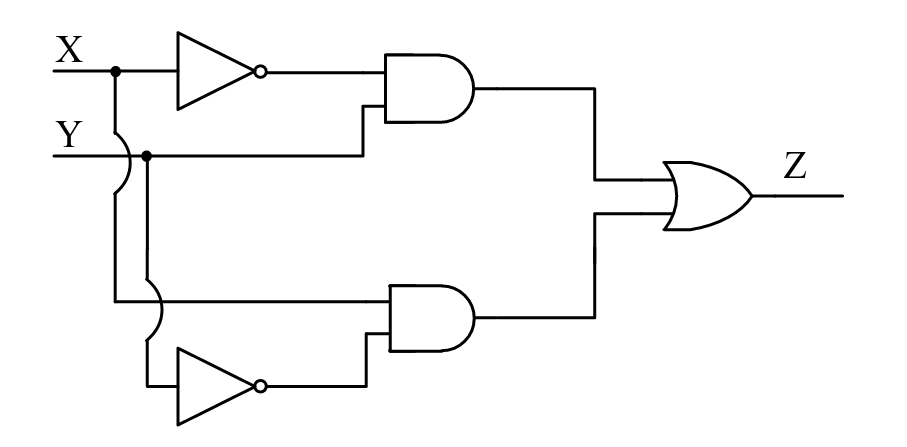
\includegraphics[width=\columnwidth]{figs/2019-gate-ee-36.png}
\caption{}
\label{fig:2019-gate-ee-36}
\end{figure}
\item 
\label{prob:2018-gate-CS-4}		
Let $\oplus$ and $\odot$ denote the Exclusive OR and Exclusive NOR operations, respectively.Which one of the following is NOT CORRECT ?
\ref{prob:2018-gate-CS-4}
\hfill (GATE CS 2018)
\begin{samepage}
\begin{enumerate}[label=(\Alph*)]
    \item $\overline{P\oplus Q}$ = $ P \odot Q $
    \item $\overline{P} \oplus Q$ = $ P \odot Q $
    \item $\overline{P} \oplus \overline{Q}$ = $ P \oplus Q $
    \item $(P \oplus \overline{P}) \oplus Q$ = $(P \odot \overline{P}) \odot \overline{Q}$
\end{enumerate}
\end{samepage}

\item A Boolean digital circuit is composed using two 4-input multiplexers $(M1 and M2)$ and one 2-input multiplexer $(M3)$ as shown in the figure. $X0$–$X7$ are the inputs of the multiplexers $M1$ and $M2$ and could be connected to either $0$ or $1$. The select lines of the multiplexers are connected to Boolean variables $A$, $B$ and $C$ as shown.\hfill(GATE CS2023,44)

\begin{figure}[H]
    \centering
        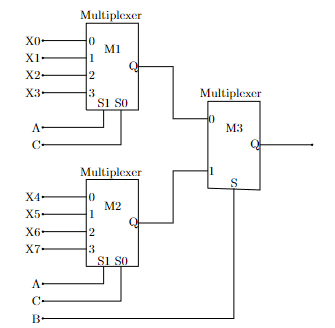
\includegraphics[width=\columnwidth]{figs/Multiplexer.png}
    \caption{Digital Circuit}
    \label{fig:Multiplexer}
\end{figure}

Which one of the following set of values of $(X0, X1, X2, X3, X4, X5, X6, X7)$ will realise the Boolean function 
$\overline{A} + \overline{A}.\overline{C}+A.\overline{B}.C $ ?
 \begin{enumerate}
     \item (1, 1, 0, 0, 1, 1, 1, 0)
     \item (1, 1, 0, 0, 1, 1, 0, 1)
     \item (1, 1, 0, 1, 1, 1, 0, 0)
     \item (0, 0, 1, 1, 0, 1, 1, 1)
 \end{enumerate}
\item For the given digital circuit, $A = B = 1$. Assume that AND, OR, and NOT gates have propagation delays of $10\mathrm{ns}$,$10\mathrm{ns}$, and $5\mathrm{ns}$ respectively. All lines have zero
propagation delay. Given that $C = 1$ when the circuit is turned on, the frequency of steady-state oscillation of the output $Y$  is  \rule{30pt}{1pt}.
\hfill (GATE IN 2023)
\begin{figure}[H]
        \centering  
        
        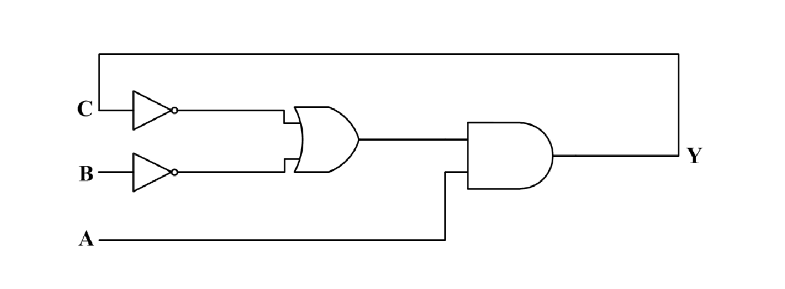
\includegraphics[width=\columnwidth]{figs/gate.png}
        \caption{Image}
	\label{fig:Image}
        
\end{figure}
    \begin{enumerate}
        \item $20 \mathrm{MHz}$
        \item $15 \mathrm{MHz}$
        \item $40 \mathrm{MHz}$
        \item $50 \mathrm{MHz}$
    \end{enumerate}
\item Select the Boolean function(s) equivalent to $x + yz$, where $x,y$, and $z$ are Boolean variables, and + denotes logical OR  operation.\hfill(GATE EC 2022)
	\begin{enumerate}[label=(\Alph*)]
		\item $x + z + {xy}$
		\item ${(x + y)}{(x + z)}$
		\item $x + {xy} + {yz}$
		\item $x + {xz} + {xy}$
	\end{enumerate}
 \item Which one of the following options is CORRECT for the given circuit ?\hfill(GATE PHYSICS 2023)
		\begin{figure}[H]
			\centering
			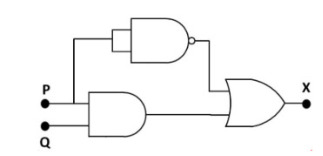
\includegraphics[width=\columnwidth]{figs/Q24.jpg}
			\caption{}
			\label{figure:xxxx}
		\end{figure}

		\begin{enumerate}[label=(\Alph*)]
		\item P = $1$, Q = $1$ ; X = $0$
		\item P = $1$, Q = $0$ ; X = $1$
		\item P = $0$, Q = $1$ ; X = $0$
		\item P = $0$, Q = $0$ ; X = $1$
	\end{enumerate}

\item In the circuit diagram shown below, the logic gates operate with a supply voltage of $1 V$. NAND and XNOR have $200$ps and $400$ps input-to-output delay, respectively.

At time $t=T.A(t)=0,B(t)=1 and Z(t)=0.$ When the inputs are changed to $A(t)=1,B(t)=0 \text{at} t=2T$, a 1 V pulse is observed at $Z$. the pulse width of the $1 V$ pulse is  ps.


\hfill{(GATE BM 2022)}

\begin{figure}[H]
\centering
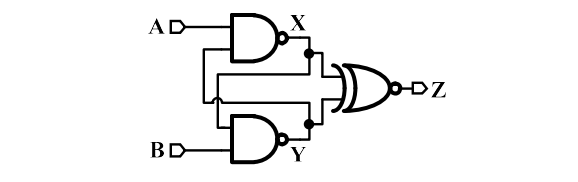
\includegraphics[width=\columnwidth]{figs/bm2022.png}
\caption{}
\label{fig:GATE Digram}
\end{figure}

\begin{enumerate}
\item $100$
\item $200$
\item $400$
\item $600$
\end {enumerate}

\item 
Consider a Boolean gate (D) where the output (Y) is related to the inputs (A) and (B) as, $Y = A + B$, where + denotes logical OR operation. The Boolean inputs '0' and '1' are also available separately. Using instances of only D gates and inputs '0' and '1', (select the correct option(s)).\hfill{(GATE EC 2022)}

\begin{enumerate}
\item  NAND logic can be implemented
\item  OR logic cannot be implemented
\item  NOR logic can be implemented
\item  AND logic cannot be implemented.
\end{enumerate}

\item Let $R1$ and $R2$ be two $4$-bit registers that store numbers in $2$’s complement form.
For the operation $R1+R2$, which one of the following values of $R1$ and $R2$ gives an
arithmetic overflow?
\hfill{(GATE CS 2022)}

    \begin{enumerate}
        \item $R1 = 1011$ and $R2 = 1110$
        \item $R1 = 1100$ and $R2 = 1010$
        \item $R1 = 0011$ and $R2 = 0100$
        \item $R1 = 1001$ and $R2 = 1111$
    \end{enumerate}


\item The maximmunm clock frequeccy in MHz of a $4$-stage ripple counter, utilize flip-flops, with each flip-flop having a propagation delay of $20$ ns, is $\rule{2cm}{0.15mm}$.\\
(\textit{round off to one decimal place})
\hfill{(GATE EE 20222)}

\item The logic block shown has an output $F$ given by \rule{2cm}{0.15mm}
\hfill{(GATE IN 2021)}
\begin{figure}[H]
\centering
\includegraphics[width=\columnwidth]{figs/gatemage.jpg}
\end{figure}
\begin{enumerate}
	\item$A+B$
	\item$A.\bar{B}$
	\item$A+\bar{B}$
	\item$\bar{B}$
\end{enumerate}

\item Consider the following Boolean expression 
\begin{align*} F = (X+Y+Z)(\bar{X}+Y)(\bar{Y}+Z) \end{align*}
       
Which of the following Boolean expressions is/are equivalent to $\overline{F}$ (complement of 
 F)?
 
\hfill{(Gate CS 2021,42)}
\begin{enumerate}                                     
\item $(\bar{X}+\bar{Y}+\bar{Z})(X+\bar{Y})(Y+\bar{Z})$
\item $X\bar{Y}+\bar{Z}$
\item $(X+\bar{Z})(\bar{Y}+\bar{Z})$
\item $X\bar{Y}+Y\bar{Z}+\bar{X}\bar{Y}\bar{Z}$ 
\end{enumerate}

    \item The propagation delays of the XOR gate, AND gate and multiplexer \brak{MUX} in the circut shown in the figure are $4 ns$, $2 ns$ and $1 ns$, respectively.
    If all the inputs $P, Q, R, S$ and T are applied simultaneously and held constant, the maximum propagation delay of the circuit is
\hfill(GATE-EC2021,31)  

\begin{figure}[H]
\begin{circuitikz}
\draw (7,1)coordinate (E) -- (8,1)coordinate (F) -- (8,-1)coordinate (G) -- (7,-1)coordinate (H) -- (7,1)coordinate (E);
\draw (11,2)coordinate (I) -- (13,2)coordinate (J) -- (13,-1)coordinate (K) -- (11,-1)coordinate (L) -- (11,2)coordinate (I);
 \draw ($(J)!0.5!(K)$)--++(0:2)node[right]{$Y$};
 \draw ($(L)!0.5!(K)$)node[anchor=south]{$S0$}--++(90:-2)--++(1:-10)node[left]{$T$};
 \draw ($(H)!0.5!(G)$)node[anchor=south]{$S0$}--++(90:-2)--++(1:0)node[left]{};
\draw (4,2) node[and port] (myand1) {};
\draw (myand1.in 1) node (A1)     [anchor=east,xshift=-1cm]           {$P$}
(myand1.in 1) -- (A1);
\draw(4,-2) node[and port] (myand2) {}
(myand2.in 2) node (B2)     [anchor=east,xshift=-1cm]           {$S$};
\draw(myand2.in 2) -- (B2);
\draw (10,0) node[and port] (myand3) {};
\draw (4,0) node[xor port] (myxor) {};
\draw (myand1.in 2) node (B1)     [anchor=east,xshift=-1cm,yshift=-.7cm]  {$Q$};
\draw (B1) -- ++(1.25cm,0);
\draw (myxor.in 1) node (B1)     [anchor=east,xshift=-1cm,yshift=-1.3cm]  {$R$};
\draw (B1) -- ++(1.25cm,0);

\draw (myand1.in 2) |- (myxor.in 1);
\draw (myand2.in 1) |- (myxor.in 2);

\draw (myxor.out) |- ($(E)!0.2!(H)$)--++(0:0)node[right]{$0$};
\draw(myand1.out) |- ($(I)!0.2!(L)$)--++ (0:0)node[right]{$0$};
\draw (myand1.out) -| (myand3.in 1);
\draw(myand3.out) -| ($(I)!0.7!(L)$)--++(0:0)node[right]{$1$};
\draw ($(F)!0.6!(G)$)--++(0:0)node[right]{} -| (myand3.in 2) ;
\draw (myand2.out) |- ($(E)!0.7!(H)$)--++(0:0)node[right]{$1$};

\end{circuitikz}
~


\caption{circuit daigram} 
\label{fig:block_diagram}
\end{figure}
\begin{enumerate}

    \item $3 ns$
    \item $5 ns$
    \item $6 ns$
    \item $7 ns$
\end{enumerate}
\item  The above combination of logic gate represent the operation
 \hfill(GATE PH 2021)
	      \begin{figure}[H]
		      \centering
		                   \begin{circuitikz}
              
                  \draw (2,5) node[not port,scale=2] (not) {};
                  \draw (not.in) -- ++(-0.5,0);
                  \draw (not.out) -- ++(0.5,0) ;
                  
                
                
                \draw (7.5,3) node[or port,scale=2] (orgate) {};
                  \draw (orgate.in 1) -- ++(-0.5,0) ;
                  \draw (orgate.in 2) -- ++(-0.5,0);
                  \draw (orgate.out) -- ++(0.5,0) ;
                
                 \draw (2,1) node[not port,scale=2] (notgate) {};
                  \draw (notgate.in) -- ++(-0.5,0) ;
                  \draw (notgate.out) -- ++(0.5,0) ;
                
                \draw (notgate.out) -- ([xshift=0.5cm]notgate.out) |-(orgate.in 2);
                  
                \draw (not.out) -- ([xshift=0.5cm]not.out) |-(orgate.in 1);
                  
            \end{circuitikz}

	              \caption{combination circuit}
	      \end{figure}

	\begin{enumerate}
       \item OR
       \item NAND
       \item AND
       \item NOR
   \end{enumerate}
\item Consider the boolean Function $z\brak{a,b,c}$ from below .
		\begin{figure}[H]
			\centering
			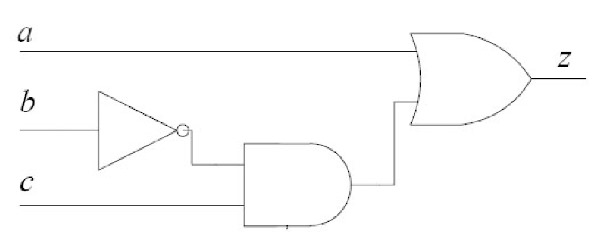
\includegraphics[width=\columnwidth]{figs/203.png}
			\caption{circuit diagram}
		\end{figure}
		
	\hfill{(Gate CS-2020)}
	
		Which of the following minterm lists represent the circuit given above?
	\begin{enumerate}
		\item $z=\Sigma\brak{0,1,3,7}$
		\item $z=\Sigma\brak{1,4,5,6,7}$
		\item $z=\Sigma\brak{2,4,5,6,7}$
		\item $z=\Sigma\brak{2,3,5}$
	\end{enumerate}	   
\item In the latch circuit shown, the NAND gates have non-zero but unequal propagation delays. The present input condition is: $P=Q=\lq 0\rq$. If the input condition is changed simultaneously to $P=Q=\lq 1\rq$,the outputs $X$ and $Y$ are 
\begin{figure}[H]
\centering
\label{figure_1}
\begin{circuitikz}
    \draw (0,0) node[nand port] (nand1) {};
    \draw (0,-2) node[nand port] (nand2) {};
    \draw (nand1.in 1) -- ++(-0.5,0) node[left] {$P$};
    \draw (nand1.in 2) -- ++(-0.2,0) coordinate (in1);
    \draw (nand1.out) -- ++(0.1,0) coordinate (out1); 
    \draw (nand2.in 1) -- ++(-0.2,0) coordinate (in2);
    \draw (nand2.in 2) -- ++(-0.5,0) node[left] {$Q$};
    \draw (nand2.out) -- ++(0.1,0) coordinate (out2);
    \draw (out2)-- ++(0,0.5)-- ++(-2,1) |- (in1);
    \draw (out1)-- ++(0,-0.5)-- ++(-2,-1) |- (in2);
    \draw (out1) -- ++(1,0) node[above right] {X};
    \draw (out2) -- ++(1,0) node[above right] {Y};
\end{circuitikz}

\end{figure}
\begin{enumerate}
\item $X=\lq 1\rq,Y=\lq 1 \rq$
\item either $X=\lq 1\rq,Y=\lq 0\rq$ or $X=\lq 0\rq,Y=\lq 1\rq$
\item either $X=\lq 1\rq,Y=\lq 1\rq$ or $X=\lq 0\rq,Y=\lq 0\rq$
\item $X=\lq 0\rq,Y=\lq 0 \rq$
\end{enumerate}
\hfill(GATE EC 2017)

\item Consider three $4$-variable functions $f_1, f_2, $and $f_3,$ which are expressed in sum-of-minterms as \newline \quad $f_1 = \sum\brak{0,2,5,8,14}$, \quad $f_2=\sum\brak{2,3,6,8,14,15}$, \quad $f_3 = \sum\brak{2,7,11,14}$ \newline For the following circuit with one AND gate and one XOR gate, the output function $f$ can be expressed as:
	\hfill(GATE-CS2019,30)
	\begin{figure}[H]
		 \centering
			\begin{circuitikz}
    % Draw AND gate
    \draw (0,0) node[and port] (and) {AND};
    
    % Draw XOR gate
    \draw (4,-0.2) node[xor port] (xor) {XOR};
    
    % Connect AND output to XOR input
    \draw (and.out) -- (xor.in 1);
    
    % Draw input wires
    \draw (and.in 1) -- ++(-1,0) node[left] {$f_1$};
    \draw (and.in 2) -- ++(-1,0) node[left] {$f_2$};
    \draw (xor.in 2)--++(-90:2) --++(-5,0) node[left] {$f_3$};    % Draw XOR output
    \draw (xor.out) -- ++(1,0) node[right] {$f$};
\end{circuitikz}


                 \caption{Circuit Daigram}
	\end{figure}
		\begin{enumerate}
		\item $\sum\brak{7,8,11}$
		\item $\sum\brak{2,7,8,11,14}$
		\item $\sum\brak{2,14}$
		\item $\sum\brak{0,2,3,5,6,7,8,11,14,15}$
		\end{enumerate}

\item In the circuit shown, what are the values of $F$for $EN=0$ and $EN=1$,  respectively?
 \hfill(GATE-EC2019,14)  

\begin{figure}[H]
    \centering
    \begin{circuitikz}

\draw (0.5,1) node[nand port] (nand) {};
\draw (nand.in 1) -- ++(-1.7,0) node[left] {};
\draw (nand.in 2) -- ++(-2.2,0) node[left] {EN};
\draw (nand.out) -- ++(0.5,0) node[midway, above] {};
\draw (0.5,-3) node[nor port] (nor) {};
\draw (nor.in 1) node[left] {};
\draw (nor.in 2) --++(-2.2,0) node[left] {D};
\draw (nor.out) -- ++(0.5,0) node[midway, above] {};
\draw (-1.6,-1) node[rotate=270,not port] (not) {};
\draw (not.in) |-(nand.in 2);
\draw  (nor.in 1) -| (not.out);
\draw (2,1) node[pmos] (pmos) {};
\draw (2,-3) node[nmos] (nmos) {};
\draw (nand.out) -- (pmos.gate);
\draw (nor.out) -- (nmos.gate);
\draw(nand.in 1) -- ++(-1.7,0) |- (nor.in 2) -- ++(-1,0);
\draw (pmos.drain) -- (nmos.drain);
\draw (pmos.drain)--++(90:-1)--++(2:1)node[left, yshift=0.2cm]{$F$};
\draw (nmos.source) -- (nmos.source |- 0,-4) node[ground] {};
\draw(2,1.7) node[rground,yscale=-1] {};
\draw(2,2.3) node(right) {$V_{DD}$};

\end{circuitikz}


    \caption{Circuit Diagram}
\end{figure}
\begin{enumerate}
    \item $0$ and $D$
    \item $Hi-Z$ and $D$
    \item $0$ and $1$
    \item $Hi-Z$ and $\overline{D}$
\end{enumerate}
\item In the circuit shown, $A$ and $B$ are the inputs and $F$ is the output. What is the functionality of the circuit?
           \hfill(GATE-EC2019,15)
           
\begin{figure}[H]
\centering

\begin{circuitikz}
    % Draw PMOS transistors
     \draw (2,1) node [pmos] (pmos1) {};
    \draw (2,0) node [pmos,rotate=180] (pmos2) {};
    \draw (0,-2) node [nmos,rotate=180] (nmos1) {};
    \draw (4,-2) node [nmos] (nmos2) {};
    
    % connections
     \draw(pmos1.gate)  -- (nmos1.gate);
      \draw(pmos2.gate) -- (nmos2.gate);
     \draw (pmos1.drain) -- (pmos2.drain);
    \draw (nmos1.source) -- (nmos2.drain);
    \draw (nmos1.gate) --(nmos2.source);
    \draw (nmos2.gate) -- (nmos1.drain);
    \draw (pmos2.source) -- (2,-1.22);
    \draw (nmos2.drain) -- (4,-1.22) node[circ]{};
    \draw (nmos2.drain)node[anchor=east,xshift=0.45cm,yshift=-0cm] 
    {$F$};
    %%B
    \draw (nmos2.source) node[circ]{};
    \draw (nmos2.source)node[anchor=east,xshift=0.48cm,yshift=-0cm] {$B$};
    %%A
    \draw (nmos1.drain)node[circ]{};
     \draw (nmos1.drain)node[anchor=east,xshift=0cm,yshift=-0cm] {$A$};
     %%vdd
    \draw (2,1.75) node[rground,yscale=-1] {};
    \draw (2.5,1.8) node(right) {$V_{DD}$};
\end{circuitikz}


\caption{Circuit Diagram}

\end{figure}
\begin{enumerate}
\item Latch
\item XNOR
\item SRAM Cell
\item XOR
\end{enumerate}

\item In the circuit shown below, assume that the comparators are ideal and all components have zero propagation delay. In one period of the input signal $Vin=6\sin\brak{\omega t}$, the fraction of the time for which the output OUT is in logic HIGH is 
		                 \hfill(GATE-IN2019,34)
\begin{figure}[H]
\centering
    \begin{circuitikz}

\draw (0,0) node[op amp] (opamp1) {};
\draw (opamp1.-)  node[left]{};
\draw (opamp1.+) node[left]{};
\draw (opamp1.out) node[right]{} ;
\draw (0,5) node[op amp] (opamp2) {};
\draw (opamp2.-)  node[left]{};
\draw (opamp2.+)  node[left]{};
\draw (opamp2.out) node[right]{};
\draw (3.5,5) node[not port] (notgate1) {};
\draw (notgate1.in) node[left] {};
\draw (notgate1.out) node[right] {};
\draw (3.5,2) node[not port] (notgate2) {};
\draw (notgate2.in) node[left] {};
\draw (notgate2.out) node[right] {};
\draw (6.5,3.5) node[and port] (andgate1) {};
\draw (andgate1.in 1) node[left] {};
\draw (andgate1.in 2)  node[left] {};
\draw (andgate1.out) node[right] {};
\draw (6.5,0.5) node[and port] (andgate2) {};
\draw (andgate2.in 1) node[left] {};
\draw (andgate2.in 2)  node[left] {};
\draw (andgate2.out) node[right] {};
\draw (8,2) node[or port] (orgate) {};
\draw (orgate.in 1) node[left] {};
\draw (orgate.in 2)  node[left] {};
\draw (orgate.out) node[right] {$out$};
\draw (andgate1.out) -| (orgate.in 1);
\draw (andgate2.out) -| (orgate.in 2);
\draw (notgate1.out) -| (andgate1.in 1);
\draw (notgate2.out) -| (andgate1.in 2);
\draw (opamp2.out) -|(notgate1.in);
\draw (opamp1.out) -| (andgate2.in 2);
\draw(opamp2.out)--++(90:0)|-(andgate2.in 1);
\draw(notgate2.in)--++(50:0)|-(opamp1.out);
\draw(opamp1.-)--++(90:0)-|(-3,2)|-(opamp2.-);
\draw(opamp2.+)--++(0,-1) node[rground,rotate=180,yscale=-1]{};
\draw (-1.2,2.8)node(right) {$3V$};
\draw(opamp1.+)--++(0,-1) node[ground,rotate=180,yscale=-1]{};
\draw (-5,5.5) to[sV] (-5,0)node[ground,rotate=180,yscale=-1]{};
\draw (-5,5.5) -- (opamp2.-);
\draw (-6,3)node(right) {$6 \sin{\omega t}$};
\draw (0,5.5) -- (0,6.2)node(right) {};
\draw (0,6.5) node(right) {$HIGH$};
\draw (0,4.5) -- (0,3.8)node(right) {};
\draw(0,3.5) node(right) {LOW};
\draw (0,0.5) -- (0,1.2)node(right) {};
\draw (0,1.5) node(right) {$HIGH$};
\draw (0,-0.5) -- (0,-1.2)node(right) {};
\draw (0,-1.5) node(right) {$LOW$};

\end{circuitikz}


	    \caption{Circuit Daigram}
     \end{figure}
\begin{enumerate}
	\item $\dfrac{1}{12}$
	\item $\dfrac{1}{2}$
	\item $\dfrac{2}{3}$
	\item $\dfrac{5}{6}$
\end{enumerate}


\item The figure below shows the $ith$ full-adder block of a binary adder circuit. $C_i$ is the input carry and $C_{i+1}$is the output carry of the circuit. Assume that each logic gate has a delay of $2$ nanosecond, with no additional time delay due to the interconnecting wires. If the inputs $A_i$ , $B_i$; are available and stable throughout the carry propagation, the maximum time taken for an input $C_i$, to produce a steady-state output $C_{i+1}$ is $\underline{\hspace{18pt}}$ nanosecond.
	               \hfill(GATE-IN2019,22)
\begin{figure}[H] 
    \centering
	\begin{circuitikz}
    \draw (0,0) node[xor port] (xor1) {};
    \draw (xor1.out)  node[right] {};
    \draw (xor1.in 1) -- ++(-0.52,0) node[left] {$B_i$};
    \draw (xor1.in 2) -- ++(-1,0) node[left] {$A_i$};
    
    \draw (5,0) node[xor port] (xor2) {};
    \draw (xor2.out) node[right] {$S_i$};
    \draw (xor2.in 1)  node[left] {};
    \draw (xor2.in 2) |- (2,-2.29) node[below] {$C_i$};
    % First AND gate
    \draw (6,-2) node[and port] (and1) {};
    \draw (and1.out) node[right] {};
    \draw (and1.in 1) node[left] {};
    \draw (and1.in 2)  node[left] {};
    
    % Second AND gate
    \draw (0,-2) node[and port] (and2) {};
    \draw (and2.out)  node[right] {};
    \draw (and2.in 1)  node[left] {};
    \draw (and2.in 2)  node[left] {};
    \draw (9,-3) node[or port] (or) {};
    \draw (or.out) -- ++(0,0) node[right] {$C_{i+1}$};
    \draw (or.in 1) -- ++(-0.5,0) node[left] {};
    \draw (or.in 2) -- ++(-0.5,0) node[left] {};
   \draw (xor1.in 1) -- ++(-0.5,0) |- (and2.in 1);
   \draw (xor1.in 2) -- ++(-1,0) |- (and2.in 2);
    \draw(xor1.out)  --++(1,0)   |- (xor2.in 1);
    \draw(xor2.in 1)--++(-2,0)   |-(and1.in 1);
   % \draw(xor2.in 2)--++(-3,0)   |-(and1.in 2);
    \draw (and1.out)--++(0,-0.7) |-(or.in 1);
     \draw (and2.out)--++(0,-0.7) |-(or.in 2);
     \draw(xor2.in 2) |-(and1.in 2);
    \end{circuitikz}



	\caption{Full Adder}
\end{figure}
\item The Boolean operation performed by the following  circuit at the output $O$ is \underline{\hspace{2cm}}
    $\hfill\brak{GATE \enspace IN2020-12}$

\begin{figure}[H]
\begin{center}



    \begin{circuitikz}[circuit logic IEC]
        
        \node[and gate, inputs={nnnn}, and gate IEC symbol={}, text height=6cm, text width=3cm] (A) at  (0,0){}; 
        \draw (-2.55,0.62) -- ++(-3.2,0);
        \draw (-2.55,-0.62) -- ++(-3.2,0); 
        \draw (-2.55,-1.85) -- ++(-5.5,0); 
        \draw (-5.7,-0.65) -- ++(0,2.5); 
        \draw (-8,-1.9) -- ++(0,3.72); 
        \node at (0.6,2.5) [anchor=north east] {4:1};
        \node at (0.8,2) [anchor=north east] {Mux};
        \node[anchor=east] at ([xshift=0.6cm]A.input 1) {$I_0$};
        \node[anchor=east] at ([xshift=0.6cm]A.input 2) {$I_1$};
        \node[anchor=east] at ([xshift=0.6cm]A.input 3) {$I_2$};
        \node[anchor=east] at ([xshift=0.6cm]A.input 4) {$I_3$};
       \draw ([xshift=-0.6cm]A.output) node[right] {$O$};

        \draw (A.output) -- ++(0.2,0); 
        \foreach \i in {1,...,4}
            \draw (A.input \i) -- ++(-1,0);
        \draw (A.output) -- ++(1,0);
        \node[not port] (not_gate) at (-4.5,1.85) {};
        \draw (not_gate.out) -- ++(1.2,0);
        \draw (not_gate.in) -- ++(-1,0);
        \node[not port] (not_gate) at (-6.9,1.85) {};
        \draw (not_gate.in) -- ++(-1.9,0);
        \draw (-9.49,-1.67) -- ++(0,3.5); 
        \draw (-9.49,-1.67) node[ground] {};
        \path (A.south) -- ++(0,-0.5) coordinate (bottom_center);
    
        \draw (A.south) ++(-0.5,0) -- ++(0,-0.5) node[below] {$s_1$};
        \draw (A.south) ++(0.5,0) -- ++(0,-0.5) node[below] {$s_0$};
      
        \node[below] at ($(A.south) + (-0.7,-0.9)$) {MSB};
       
        \node[below] at ($(A.south) + (0.7,-0.9)$) {LSB};
    \end{circuitikz}
\end{center}
\caption{Circuit Diagram}
\label{fig:figure13}
\end{figure}

\begin{enumerate}

            \item  $O=S_1\oplus S_0$ 
            
            \item  $O=S_1\bullet\overline{\rm S_0}$
            
            \item  $O=S_1 + S_0$
            
            \item $O=S_0\bullet\overline{\rm S _1}$
 \end{enumerate}
\item  The chip select logic for a certain DRAM chip in a memory system design is shown below. Assume that the memory system has 16 address lines denoted by ${A_{15}}$ to ${A_0}$. What is the range of addresses (in hexadecimal) of the memory system that can get enabled by the chip select (CS) signal?
\hfill{\brak{GATE \enspace CS2019-2}}

\begin{figure}[H]
\begin{center}
\begin{circuitikz}
\draw ((5,5) node[ieeestd and port,number inputs=5,minimum height=5cm, minimum width=5cm, anchor=in 1] (B) {} (B.in 1) node[anchor=east] {$A_{15}$}(B.in 2) node[anchor=east] {$A_{14}$}(B.in 3) node[anchor=east] {$A_{13}$}(B.in 4) node[anchor=east] {$A_{12}$}(B.in 5) node[anchor=east] {$A_{11}$}(B.out) node[anchor=west] {$CS$};
\node at (B.bin 3) [ocirc, left]{} ;
\node at (B.bin 4) [ocirc, left]{};
\end{circuitikz}  
\end{center}
\caption{Logic Diagram}
\label{fig:figure14}
\end{figure}

\begin{enumerate}
\item ${C800}$ to ${CFFF}$
\item ${CA00}$ to ${CAFF}$
\item ${CA00}$ to ${C8FF}$
\item ${DA00}$ to ${DFFF}$
\end{enumerate}  


\item A $6{\frac{1}{2}}$ digit time counter is set in the time period mode of operation and range is set as 'ns'. For an input signalthe time-counter displays $1000000$. with the same input signal,The time countr is changed to 'frequency' mode of operation and the range is set as 'HZ'.The display will be show the number$\underline{\hspace{2cm}}$.
\hfill{\brak{GATE \enspace IN2020-43}}


\item  A $2\times2$ ROM array is built with the help of diodes as shown in the circuit below. Here $W0$ and $W1$ are signals that select the word lines and $B0$ and $B1$ are signals that are output of the sense amps based on the stored data corresponding to the bit lines during the read operation.

\begin{figure}[H]
        \centering
        \begin{circuitikz} 
\draw (2,0) node[nmos] {} (3,0)
(4,0) node[nmos] {} (5,0)
(4,-0.375) node[ground] {}
(2,-0.375) node[ground] {}
;
\ctikzset{diodes/scale=0.6} 
\draw  (1,3) to[empty diode] (2,2.25)
(3,1.5) to[empty diode ] (4,0.75)
;
\ctikzset{diodes/scale=1} 

\draw [very thick](1.75,3.75) -- (2,4.25) -- (2.25,3.75) -- cycle
(3.75,3.75) -- (4,4.25) -- (4.25,3.75) -- cycle
(0,0) -- (2,0) -- (5,0)
(0,1.5) node[anchor=east] {W1}--  (5,1.5)
(0,0) -- (0,0.625)
(-0.25,1.2) node[anchor=north] {VDD}
(2,4.25) -- (2,4.6) node[anchor=south] {B0}
(4,4.25) -- (4,4.6) node[anchor=south] {B1}
(-0.15,0.55) -- (0,0.625) --(0.15,0.7)
(0,3) node[anchor=east] {W0}  -- (5,3)
(2,0.25) --  (2,3.75)
(4,0.25) -- (4,3.75)
(8.125,1.75) -- (8,1.75) -- (8,3) --(8.125,3)
(9.625,1.75) -- (9.75,1.75) -- (9.75,3) --(9.625,3);
\node (mynode) at (3,4) {\scalebox{0.5}{Sense amps}};
 \filldraw[fill=black, draw=black] (1,3) circle [radius=0.1];
 \filldraw[fill=black, draw=black] (2,2.25) circle [radius=0.1];
 \filldraw[fill=black, draw=black] (3,1.5) circle [radius=0.1];
 \filldraw[fill=black, draw=black] (4,0.75) circle [radius=0.1];
 %matrix code
\node at (8.5,3.5) {$B_{0}$};
\node at (9.25,3.5) {$B_{1}$} ;
\node at (7.4,2.75) {$W_{0}$};
\node at (8.5,2.75) {$D_{00}$};
\node at (9.25,2.75) {$D_{01}$};
\node at (7.4,2) {$W_{1}$};
\node at (8.5,2) {$D_{10}$};
\node at (9.25,2) {$D_{11}$};
\node at (8.7,1) {Bits stored in the ROM Array};


\end{circuitikz}

        \caption{ 2×2 ROM array}
     
\end{figure}
	\hfill(GATE EC2018,32)

		During the read operation, the selected word line goes high and the other word line is in a high impedance state. As per the implementation shown in the circuit diagram above, what are the bits corresponding to $D_{ij}\brak{\text{where $i=0$ or $1$ and $j=0$ or $1$}}$ stored in the ROM?
\begin{enumerate}
    \item \myvec{1 & 0\\0 & 1}
    \item \myvec{0 & 1\\1 & 0}
    \item \myvec{1 & 0\\1 & 0}    
    \item \myvec{1 & 1\\0 & 0}
\end{enumerate}

\item The two inputs A and B are connected to to an R-S latch via two AND gates as shown in the figure. If $A=1$ and $B=0$, the output $Q\bar{Q}$ is
    \begin{figure}[H]
        \centering
        \begin{circuitikz}
    %input nodes
  \draw (0,0) node[circ] (A) {};
  \draw (0,-0.6) node[circ] (Qb) {};
  \draw (0,-1.6) node[circ] (Q) {};
  \draw (0,-2.2) node[circ] (B) {};
      \draw (A) ++(180:0.5) node {A};
      \draw (Qb) ++(240:0.5) node {$\bar{Q}$};
      \draw (Q) ++(210:0.5) node {Q};
      \draw (B) ++(200:0.5) node {B};    
  %and Gate
  \draw (2,-0.3) node[and port] (anda){};
  \draw (A) -- (anda.in 1);
  \draw (Qb) -- (anda.in 2);
  \draw (2,-1.9) node[and port] (andb){};
  \draw (Q) -- (andb.in 1);
  \draw (B) -- (andb.in 2);
  
  %latch
  \draw (4,-1.1) node[flipflop SR] (SR) {\tiny R-S Latch};
  \draw (anda.out) |- (SR.pin 1);
  \draw (andb.out) |- (SR.pin 3);
  
  \draw (Qb) to ++(-1,0) to[crossing] ++(0,-2) to ++(7,0) to[short,-*] ++(0,0.65) |- (SR.pin 4);
  \draw (0,-1.6) to ++(-1.5,0) to ++(0,+2) to ++(7.5,0) to[short,-*] ++(0,-0.65) |- (SR.pin 6);
  
   \end{circuitikz}
       \end{figure}
       \hfill(GATE IN2017,43)
    \begin{enumerate}
   		\item $00$ 
   		\item $10$ 
   		\item $01$ 
   		\item $11$ 
   
   \end{enumerate}


\end{enumerate}


